\documentclass{article}
\usepackage{graphicx}
\usepackage{amsmath}
\usepackage{amssymb}
\usepackage{tabto}
\usepackage{amsfonts}
%\usepackage{MnSymbol}
\usepackage{wasysym}
\usepackage{amsthm}
\usepackage{indentfirst}
\usepackage[utf8x]{inputenc}
\usepackage{caption}
\usepackage{subcaption}
\usepackage{adjustbox}
\usepackage{verbatim}
\usepackage{tikz, pgfplots}
\usepackage{tkz-euclide}
\usepgfplotslibrary{fillbetween}
\usepackage{multicol}
\usepackage{enumitem}
\usepackage{relsize}
\usepackage{xfrac}
\usepackage{array}
\usepackage{enumitem}
\usepackage{graphicx}
\usepackage[english]{babel}
\usepackage{fancyhdr}

\newtheorem{theorem}{Theorem}[section]
\newtheorem{corollary}{Corollary}[theorem]
\newtheorem{lemma}[theorem]{Lemma}

\graphicspath{ {images/} }


%\renewcommand{\v}{\vec{v}}
%\renewcommand{\u}{\vec{u}}
%\renewcommand{\w}{\vec{w}}


\setlength\parindent{0pt}
\addtolength{\oddsidemargin}{-.875in}
\addtolength{\evensidemargin}{-.875in}
\addtolength{\textwidth}{1.75in}
\DeclareMathOperator{\im}{im}
\DeclareMathOperator{\Aut}{Aut} 
\DeclareMathOperator{\Span}{span}
\DeclareMathOperator{\End}{End}
\DeclareMathOperator{\lcm}{lcm}
\DeclareMathOperator{\Int}{int}
\DeclareMathOperator{\If}{if}
\DeclareMathOperator{\Or}{or}
\DeclareMathOperator{\Nd}{and}
\DeclareMathOperator{\st}{such\ that}
\DeclareMathOperator{\writhe}{writhe}
\DeclareMathOperator{\R}{\mathbb{R}}
\DeclareMathOperator{\PP}{\mathbb{P}}
\font\msbmx=msbm10 at 10pt
\textfont15=\msbmx
\mathchardef\subsetneqq="3F24
\mathchardef\subsetneq="3F28
\mathchardef\supsetneq="3F29

\newcommand\inv[1]{#1\raisebox{1.15ex}{$\scriptscriptstyle-\!1$}}
\newcommand{\pn}[1]{\left( #1 \right)}
\newcommand{\bk}[1]{\left[ #1 \right]}
\newcommand{\set}[1]{\left\{ #1 \right\}}
\newcommand{\vc}[1]{\left\langle #1 \right\rangle}
\newcommand{\abs}[1]{\left\lvert #1 \right\rvert}
\newcommand{\norm}[1]{\left\lVert #1 \right\rVert}
\newcommand{\mat}[1]{\ensuremath{ \begin{bmatrix} #1 \end{bmatrix} }}

\newcommand{\ansbox}[2]{\raisebox{-.5\height}{\framebox(#1,#2){}}}




\addtolength{\topmargin}{-.875in}
\addtolength{\textheight}{1.75in}
\pgfplotsset{soldot/.style={color=black,only marks,mark=*},
	holdot/.style={color=black,fill=white,only marks,mark=*},
	compat=1.12}
\pagestyle{fancy}
\lhead{Math 34A, UCSB}
\rhead{Summer 2022}

\pagenumbering{gobble}
\begin{document}
\newtheorem*{theorem*}{Theorem}


	\centerline{\Large{ Quiz 8}}\vspace{12 pt}
	\begin{tabular}{ll}
    {\bf Name}: \ansbox{230}{35} %\hspace{1.8in} 
    & {\bf Perm Number}: \ansbox{120}{35} 
    \end{tabular} \\ \\
	
	
	
In the following two problems, the function $h(t) = 40t-5t^2$ describes the height (in meters) of a ball above the ground at $t$ seconds. 
\bigskip

Interpret the following information in words by filling in the blank with \textbf{one word} that completes the sentence:
$$ h'(2)=20 \qquad h(1)=35$$
{\Large 1)} $20$ is the \ansbox{160}{35} of the ball at $2$ seconds.

{\Large 2)} $35$ is the \ansbox{160}{35} of the ball at $1$ seconds.
\bigskip
	
	%\pagebreak
{\Large 3)} A rectangular field is surrounded by a fence. The fence is divided into 4 equal parts by 3 more dividing fences all parallel to one side of the field. The field must have an area of 1000 m${}^2$. Write the perimeter as an expression \textbf{using only $\mathbf{L}$.}
	\begin{center}
	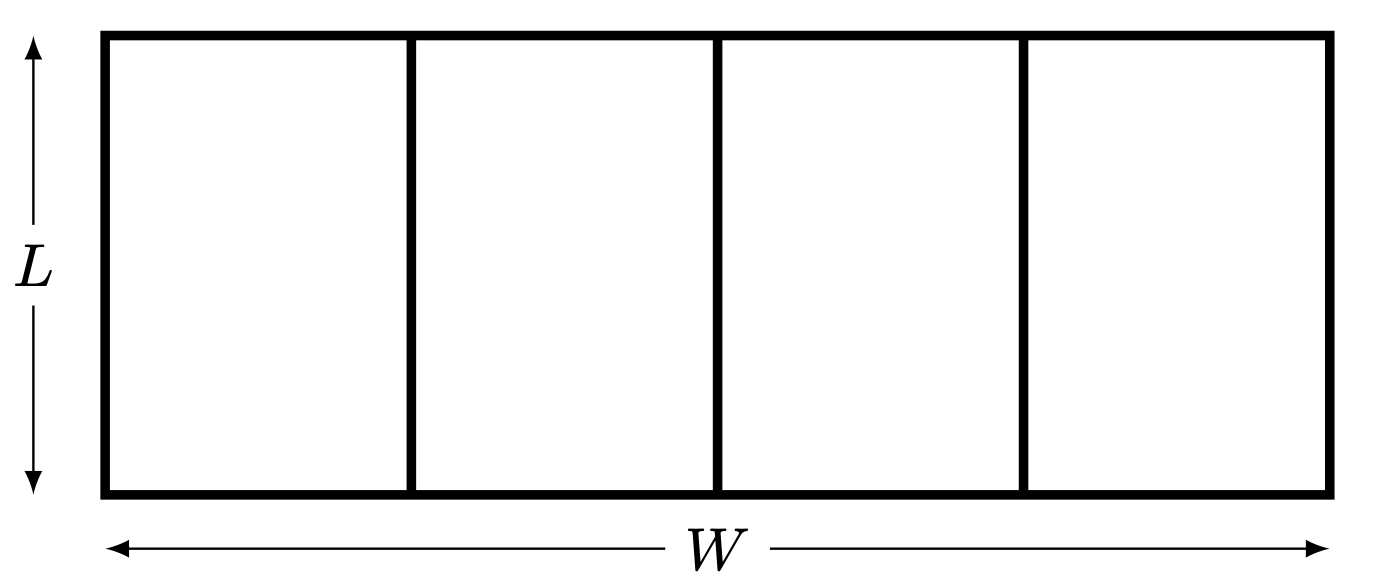
\includegraphics[width=.4\textwidth]{quiz_8_prob_3}
	\end{center}

    \vfill 
    \hfill $P=\quad$\ansbox{160}{35}
	\vspace*{.25 in}
	
    

	
\end{document}
	